\section{Durchführung}
\label{sec:Durchführung}
Die Durchführung des Versuchs zur Messung der Suszeptibilität paramagnetischer Substanzen unterteilt sich in die Messung der Filterkurve des Selektivverstärkers und in die Messung der Suszeptibilität der ausgewählten Stoffe.
\subsection{Messung der Filterkurve}
Für die Bestimmung der Filterkurve des Selektivverstärkers werden ein Sinusgenerator, der Selektivverstärker und ein Voltmeter in Reihe geschaltet. Mit dieser Schaltung misst man die Ausgangsspannung $U_\text{A}$ in Abhängigkeit von der Frequenz bei konstanter Eingangsspannung $U_E$. Dabei wird am Sinusgerator die Frequenz variiert. Die am Selektivverstärker eingestellte Durchlassfrequenz in diesem Versuch beträgt $\SI{35}{\kilo\hertz}$. Daher werden rund um die $\SI{35}{\kilo\hertz}$ vergleichsweise viele Messwerte aufgenommen. Die am Selektivverstärker eingestellte Güte beträgt hier 50.
\subsection{Messung der Suszeptibilität ausgewählter Stoffe} 
Die Messung der Suszeptibilität der Seltenen-Erd-Elemente erfolgt mit der in \autoref{fig:schaltbild} dargestellten Grundschaltung. Im durchgeführten Versuch werden die 10fach-Linearverstärker sowie das Oszilloskop nicht genutzt, da auch ohne diese eine Aufnahme brauchbarer Messwerte gelingt. Die genutzte Brückenschaltung entspricht der in \autoref{sec:mess} beschriebenen Anordnung. 
\begin{figure}[H]
    \centering
    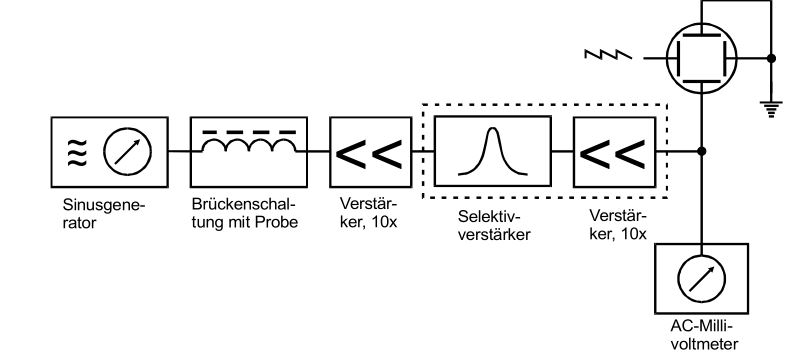
\includegraphics[width=\textwidth]{content/schaltbild.jpg}
    \caption{Blockschaltbild der Messapparatur zur Messung der Suszeptibilität ausgewählter Stoffe \cite{versuchsanleitung}}
    \label{fig:schaltbild}
  \end{figure}

  
Mit dieser Anordnung wird die Brücke zuerst ohne Probe abgeglichen. Dann wird die Probe eingeführt und die Spannung notiert. Anschließend wird die Brücke mit Probe abgegelichen. Nach jedem Abgleich werden die entsprechenden Widerstands- und Spannungswerte dokumentiert. Im durchgeführten Versuch sind die so untersuchten Elemente $\symup{Dy_2O_3}$ und $\symup{Gd_2O_3}$. Um die Messungenauigkeiten zu verringern wurde der beschriebene Messvorgang für beide Elemente 3 mal durchgeführt. 
